\begin{slikaDesno}{fig/BG.pdf}[fig/BG-kolo.pdf]
\noindent
{\color{red}*}\PID
На слици \ID.1 је приказана једна 
конструкција 
балистичког галванометра (БГ), 
инструмента за мерење протока 
наелектрисања. Казаљка инструмента
може да прави угаони отклон у границама
$0 \leq \upphi \leq \dfrac{\uppi}{2}$. Веза између струје, 
$i = i(t)$, на 
једином електричном приступу БГ
и угаоног отклона казаљке,
$\upphi = \upphi(t)$, 
дата је диференцијалном једначином
$
J \dfrac{\de^2 \upphi}{\de t^2}
+
F \dfrac{\de \upphi}{\de t}
+
K \upphi = \upalpha i,
\vspace*{1mm}
$ при чему је познато
$J = 6
\unit{s^2}$, 
$F = 24
\unit{s}
$, 
$K = 24$ и 
$\upalpha = \uppi{\rm e}
\unit{\dfrac{1}{\rm \upmu A}} \vspace*{1mm}$,
где је $\rm e$ основа природног логаритма.
Сматрати да се тај приступ
БГ, y електричном смислу, понаша као савршен кратак спој. Инструмент се калибрише на основу огледа са слике 2. 
Непосредно пре затварања прекидача, 
кондензатор је оптерећен количином наелектрисања 
$Q_0 = 1\unit{\upmu C}$
а казаљка БГ мирује у нултом положају,
$\upphi = 0$. (а)
Решавањем
у временском домену одредити 
кретање казаљке, 
$\upphi(t)$, по затварању прекидача до успостављања
новог стационарног стања.
(б) Скицирати 
временски дијаграм
$\upphi(t)$.
\end{slikaDesno}
(в) Израчунати 
вредности 
једнако размакнутих подеока са слике 1,
$Q_1$, $Q_2$, \ldots, $Q_6$,
ако се као показивање инструмента
(односно, количина 
наелектрисања протекла у импулсу) очитава вредност 
на коју показује казаљка у тренутку када је \myul{најдаље} од 
нултог подеока током свог кретања.\\

\textsc{\underline{Решење:}} На основу резултата задатка \ref{ID:capID}, струја која протиче кроз 
БГ по затварању прекидача је $i(t) = Q_0 \updelta(t)$. Та импулсна побуда побуђује разматрани систем 
па је потребно потражити одзив на побуду. 

Карактеристични полином диференцијалне једначине система је 
$P(\uplambda) = J\uplambda^2 + F\uplambda + K$, корени карактеристичног полинома потражују се 
из обрасца решења квадратне једначине као 
$\uplambda_{1,2} = \dfrac{ -F \pm \sqrt{F^2 - 4JK} }{2J}$. Заменом бројних вредности установљава
се да постоји \textit{двоструки} реални корен $\uplambda_0 = -2\unit{s^{-1}}$. На основу тога, 
општи облик одзива на импулсну побуду се може записати у облику 
\begin{equation}
    \upphi(t) = (\Upphi_0 + \Upphi_1 t) \ee^{\uplambda_0 t}, \quad
    \text{где  су $\Upphi_0$ и $\Upphi_1$ произвољне константе}
    \label{eq:phi1}
\end{equation}
Користећи поступак за одређивање одзива на импулсну побуду 
из додатка 
\ref{a:impulsni_odziv}, закључујемо да одзив треба да има прекид у изводу првог реда, а да су 
остали изводи непрекидни. На основу тога је $\upphi(0^+) = 0$ и 
$\upphi'(0^+) = \dfrac{\upalpha Q_0}{J}$.

Из израза \eqref{eq:phi1} је $\upphi(0^+) = \Upphi_0$ па је 
$\Upphi_0 = 0$. Имајући то у виду, први извод отклона казаљке у нули је 
$\upphi'(t) = \Upphi_1 \ee^{\uplambda_0 t}( \uplambda_0 t + 1 ) \Rightarrow 
\upphi'(0^+) = \Upphi_1
$, одакле се налази да је  
$\Upphi_1 = \dfrac{\upalpha Q_0}{J}$, па је 
$\Upphi_1 =  \dfrac{\uppi \ee}{6} \unit{s^{-1}}$. Коначно је тражени облик угаоног отклона казаљке 
дат изразом, $\upphi(t) = \dfrac{\upalpha Q_0}{J} t \ee^{\uplambda_0 t}$, односно бројевно 
$\upphi(t) = \dfrac{\uppi\ee}{6}\unit{s^{-1}} t 
\ee^{-2\unit{s^{-1}} t}$.  


(б) За цртање временског дијаграма најважнија је максималну тренутну вредност сигнала, будући
да се она користи у другом делу задатка. 
нуле првог извода налазе се из ранијег резултата 
$\upphi'(t) = \Upphi_1 \ee^{\uplambda_0 t_{\rm m}} (\uplambda_0 t_{\rm m} + 1) = 0$ 
одакле је $t_{\rm m} = -\dfrac{1}{\uplambda_0} = \dfrac{1}{2}\unit{s}$ а максимална 
вредност је $\upphi_{\rm m} = \dfrac{\uppi}{12}\unit{rad}$. Додатно, могуће је одредити 
и тачку превоја за прецизније цртање, решавањем $\upphi''(t) = 0$ добија се да је тренутак превоја
$t_{\uppi} = 1\unit{s}$. Временски дијаграм тог резултата приказан је на слици 
\ref{fig:\ID.3}.

\begin{figure}[ht!]
    \centering
    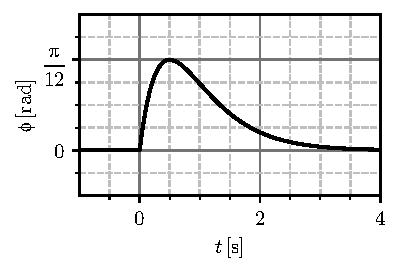
\includegraphics[scale = 1]{fig/BG_plot.pdf}
    \caption{}
    \label{fig:\ID.3}
\end{figure}

(в) Пошто је дати систем линеаран (описан је линеарном диференцијалном једначином), 
важи да уколико је побуда $1\unit{\upmu C} \updelta(t)$ произвела одзив 
$\upphi(t)$, онда ће побуда облика $k \unit{\upmu C} \updelta(t)$ произвести одзив
облика $k \upphi(t)$. Пошто је $\max k\upphi(t) = k \max \upphi(t) = \dfrac{k\uppi}{12}$,
а подеоци су размакнути за по тачно $\dfrac{\uppi}{12}$, то подеоци треба да буду 
${Q_k = k\unit{\upmu C}}$.

\vfill
